\documentclass[a4paper,12pt]{article}

\usepackage[T2A]{fontenc}
\usepackage[utf8]{inputenc}
\usepackage[english]{babel}

\usepackage[left = 2cm, right = 2cm, bottom= 2cm, top =2cm]{geometry}

\usepackage{amsmath,amsfonts,amssymb,amsthm,mathtools}
\usepackage{graphicx}
\usepackage{wrapfig}

\author{Koveshnikov Grigory}
\title{Determination Young`s modulus using acoustic resonance}
\date{\today}
\begin{document}
\maketitle
\textbf{Goal of the work:} research the phenomena of acoustic resonance in a thin rod; measure velocity of spreading of longitudinal acoustic oscillation in thin rods made up of different metals and various sizes; measure Young`s modulus of different materials.
\begin{center}
\Large{Inception}
\end{center}
Theoretical part: 


Measured parameters of rods and data was entered in the table. Using equation of 
После настройки установки: поместили стержень между двумя пластинами на минимальном расскоянии от них, причем так, чтобы концы стержня были строго посередине платформ и никак не касались их. Оценим частоты по формуле:





 

\begin{table}
\caption{frequencies for different rods}
\begin{center}
\begin{tabular}{|c|c|c|c|c|c|}
\hline 
n & 1 & 2 & 3 & 4 & 5 \\ 
\hline 
copper \( \nu \), kHz & 3.160 & 6.438 & 9.512 & 12.700 & 15.822 \\ 
\hline 
steel \( \nu \), kHz & 4.126 & 8.313 & 12.391 & 16.550 & 20.647 \\ 
\hline 
aluminum \( \nu  \), kHz & 4.2441 & 8.537 & 12.7018 & 16.970 & 21.206 \\ 
\hline 
\end{tabular}
\end{center}
\end{table}

\begin{table}
\caption{parameters of rods:}
\begin{center}
\begin{tabular}{|c|c|c|c|c|c|}
\hline 
\multicolumn{6}{|c|}{copper}\\ 
\hline 
\( d \), mm & 11.95 & 11.72 & 11.97 & 11.94 & 11.85  \\ 
\hline 
\( l \), mm & 39.6 & 40.2 & 30.2 & 40.5 & 30.3 \\ 
\hline 
\( m \), g & 39.42 & 38.74 & 30.13 & 40.38 & 29.478 \\ 
\hline 
\multicolumn{6}{|c|}{steel} \\ 
\hline 
\( d \), mm & 11.86 & 11.97 & 11.99 & 11.97 & 12.23 \\ 
\hline 
\( l \), mm & 41.4 & 40.0 & 30.0 & 29.7 & 31.4 \\ 
\hline 
\( m \), g & 37.16 & 35.16 & 26.17 & 26.03 & 28.12 \\ 
\hline 
\multicolumn{6}{|c|}{duralumin} \\
\hline 
\( d \), mm & 11.84 & 11.58 & 12.03 & 11.71 & 12.13  \\ 
\hline 
\( l \), mm & 30.2 & 40.3 & 30.1 & 30.3 & 41.4 \\ 
\hline 
\( m \), g & 9.19 & 11.79 & 9.493 & 9.00 & 13.24 \\
\hline 
\end{tabular} 
\end{center}
\end{table}

Построим графики зависимости частоты от номера гармоники по данным из таблицы для 3 стержней:\\
\begin{center}
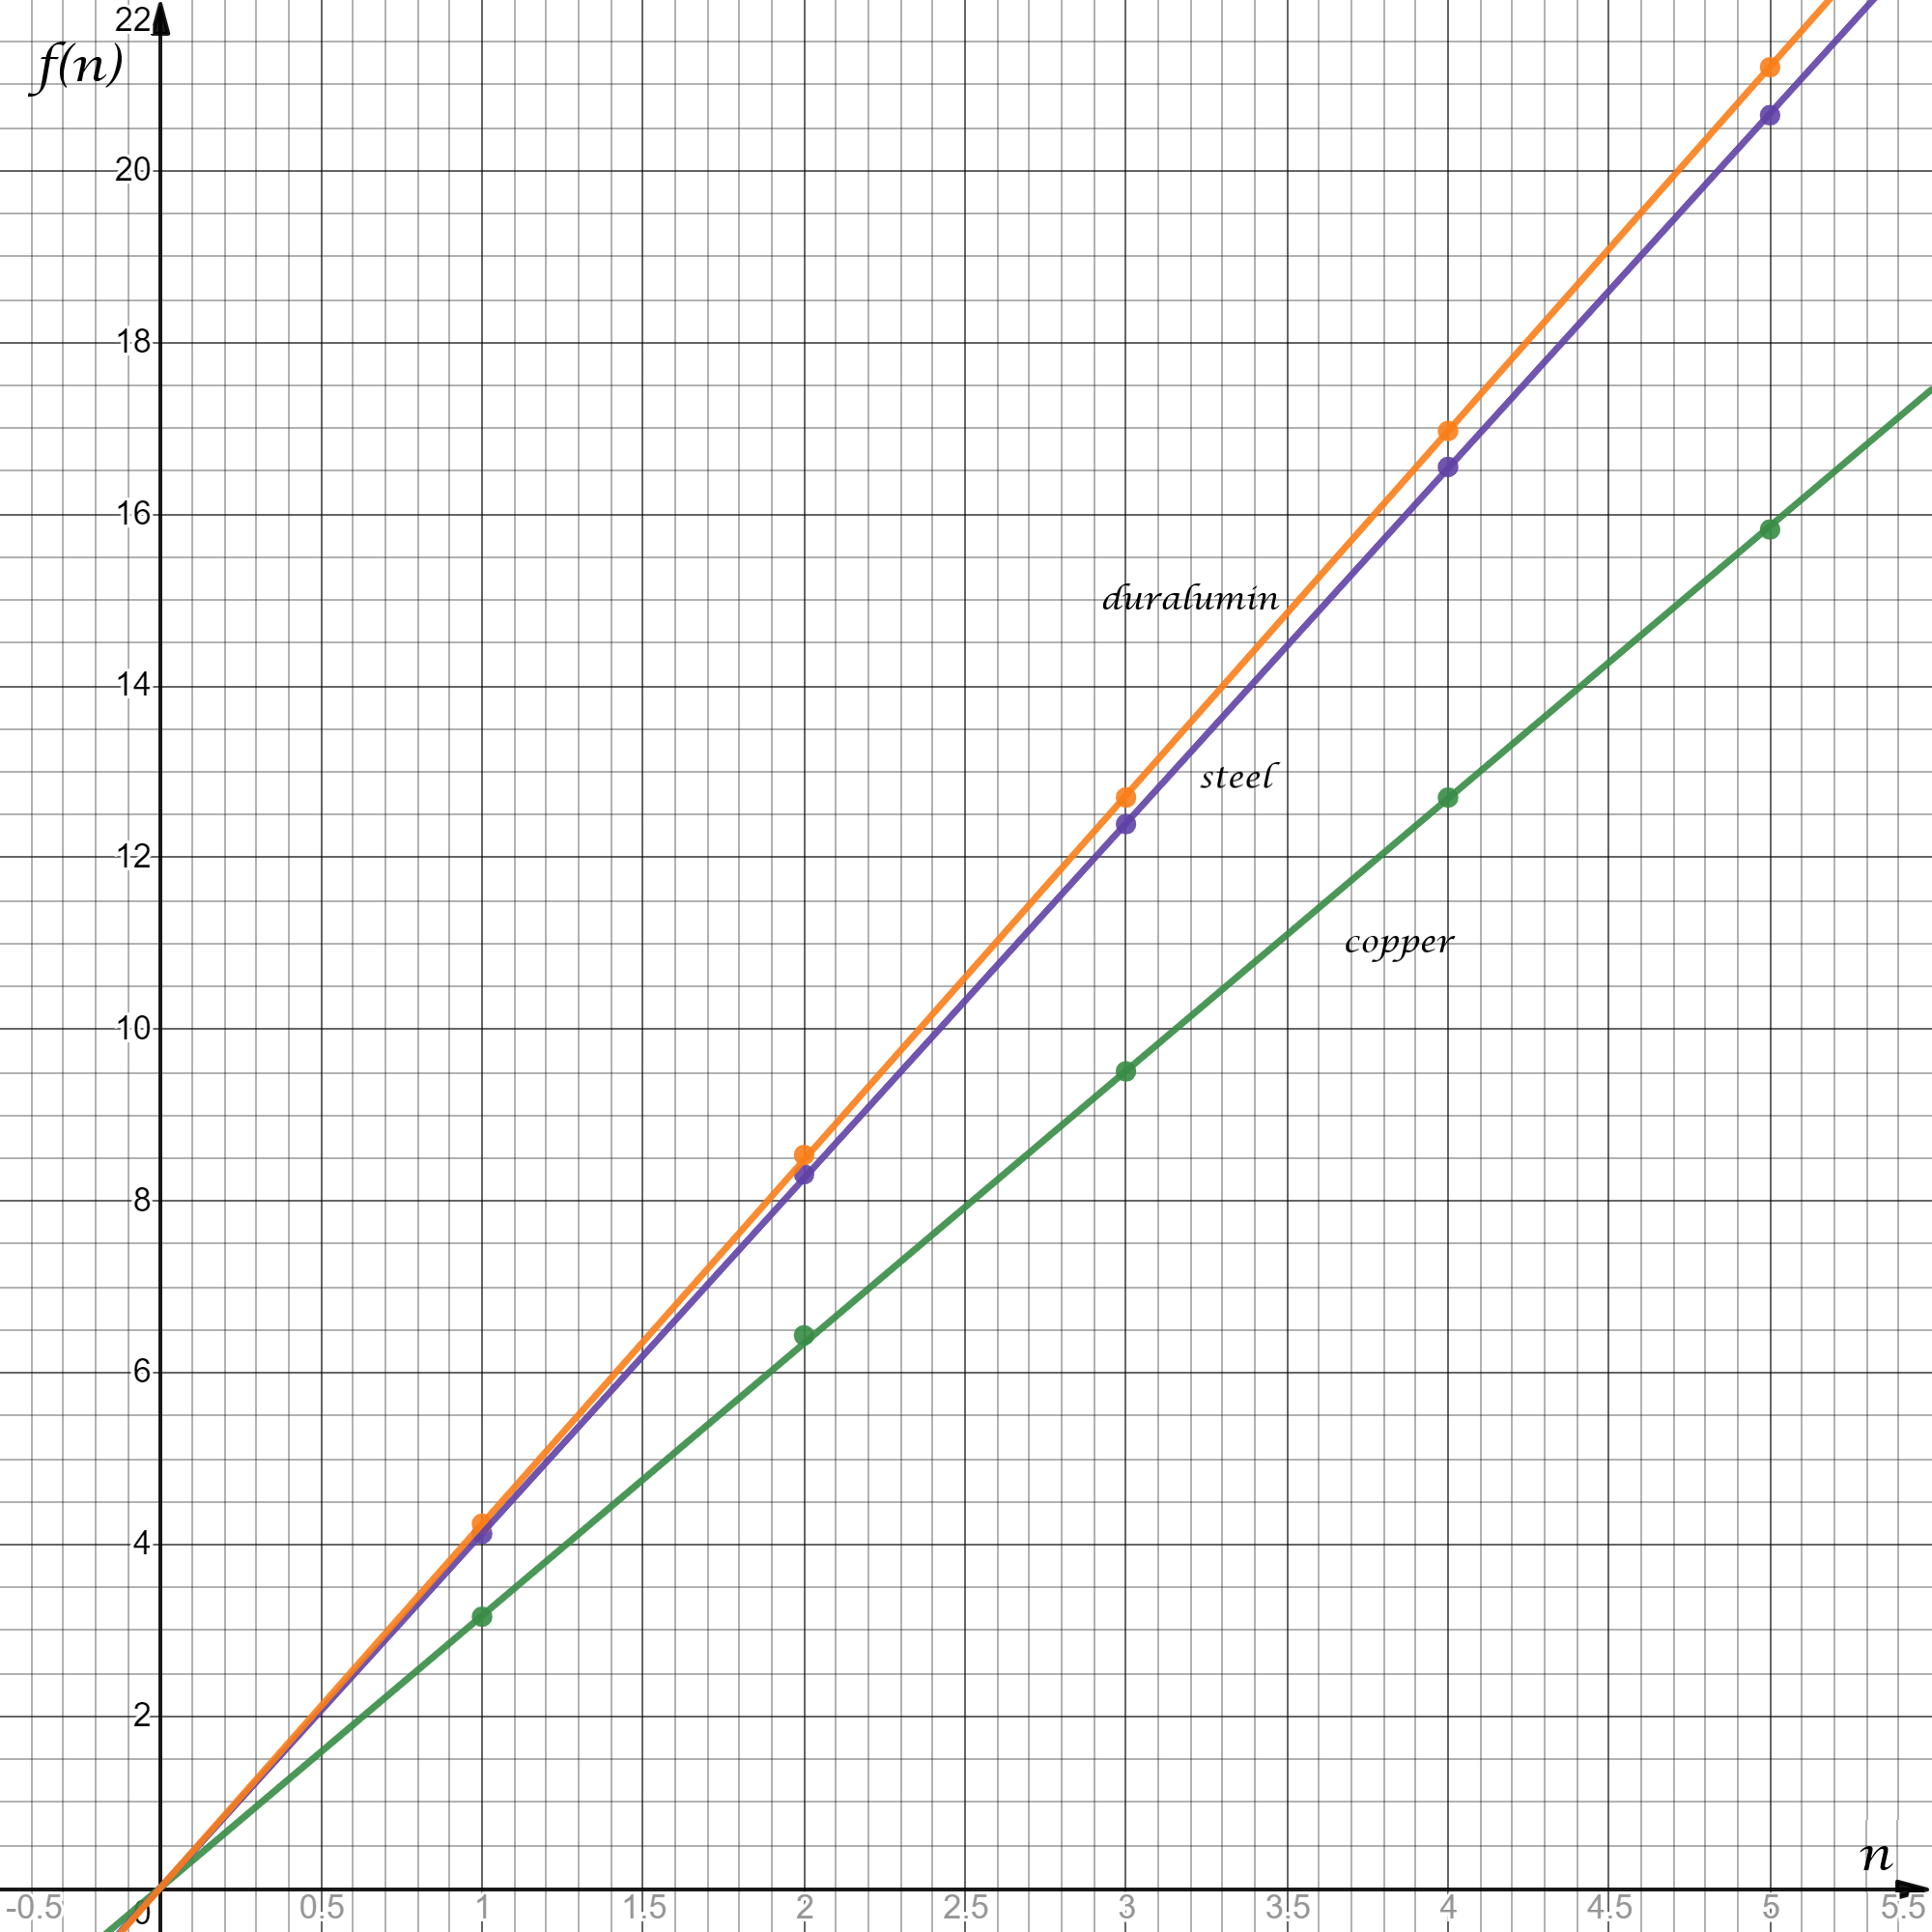
\includegraphics[scale = 0.3]{1.4.8.1.png}
\end{center}


Найдем коэффициенты по методу наименьших квадратов. Найдем из них модуль Юнга. Учитываем системетическую и случайную погрешности:\\
\(f_n = \frac{u}{2L}\cdot n\)\\
Random error:\\
\(u = 2L\dfrac{\langle f_n n \rangle}{\langle n^2 \rangle}\)\\
\(\sigma_{u} = 2L\dfrac{1}{\sqrt{5}}\sqrt{\dfrac{\langle f_n^2 \rangle}{\langle n^2 \rangle} - \left(\dfrac{u}{2L}\right)^2} \)\\

System error:\\
\(\sigma_u = \sqrt{\left(\dfrac{\sigma_L}{L}\right)^2 + \left(\dfrac{\sigma_f}{f} \right)^2} \)\\

General error:
\(\sigma_u = \sqrt{\sigma_{rand}^2 + \sigma_{syst}^2}\)
Put velocities and all errors into the table:
Enter wave velocities and their errors for 3 rods in the table:\\


\begin{tabular}{|c|c|c|c|c|}
\hline 
\(*10^3\) & \(u\) & \(\sigma_{rand} \) & \(\sigma_{syst} \) & \(\sigma_u\) \\ 
\hline 
copper & 3.172 & 0.006 & 0.002 & 0.006 \\ 
\hline 
steel & 4.134 & 0.003 & 0.002 & 0.004 \\ 
\hline 
aluminum & 4.242 & 0.004 & 0.002 & 0.004 \\ 
\hline 
\end{tabular} 
 











\end{document}